\chapter{Il Nobel per la Matematica}
Fisica, chimica, medicina, letteratura, economia e mate... NO! Tra tutte le scienze proprio la matematica, quella che Gauss aveva definito la Regina della scienze e che Galileo aveva definito il Linguaggio dell'Universo, viene esclusa dal florilegio delle declinazioni del famoso premio. Ma perchè? Perchè non esiste il Nobel della Matematica?

\section{Nobel per la matematica}
\marginpar{
	\captionsetup{type=figure}
	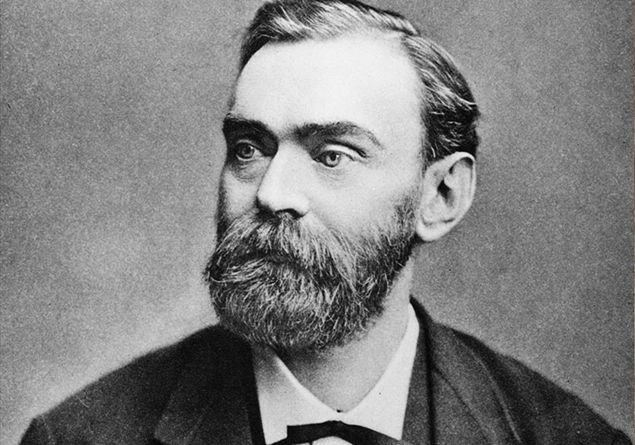
\includegraphics[width=\marginparwidth]{Nobel}
	\caption[Ritratto di Alfred Nobel]{Ritratto di Alfred Nobel}
	\label{fig:AlfredNobel}
}

Come mai non c’è il Nobel per la matematica?

Beh la domanda sorge abbastanza spontanea e anche con un po' di perplessità e amarezza. Facciamo dunque un passo indietro e capiamo dove nasce il famoso premio...

Il premio prende il nome da Alfred Nobel, l’industriale e chimico svedese che ha inventato la dinamite. È stato lui, con le sue ultime volontà, a istituire il prestigioso riconoscimento. Ma perché? La filantropia non sempre si può spiegare, ma nel caso di Nobel forse sì.

La storia, abbastanza veritiera dato che è comprovata da numerose fonti autorevoli, dice che Nobel era negli ultimi anni della sua vita tormentato da avere creato un tale strumento distruttivo... Come se ciò non bastasse, alla morte del fratello nel 1888 la stampa, avendo scambiato il celebre Alfred con il fratello Ludvig, sentenziò a caratteri cubitali "Morto il mercante di morte". Al senso di colpa si aggiungeva quindi anche il danno d’immagine.

Il denaro può dunque migliorare l'opinione che la gente ha di te? Beh a posteriori si direbbe di si! Fu dunque istituito un premio a favore di chi fosse riuscito a apportare «considerevoli benefici all’umanità».

Nobel per la matematica
La leggenda si mischia alla storia

La domanda iniziale rimane comunque ancora aperta... Perchè tra tutte le vie in cui qualcuno potrebbe migliorare la vita dell'Umanità, non ci sarebbe la Matematica?! Leggenda vuole che il signor Nobel l'abbia esclusa per gelosia: sua moglie l'avrebbe tradito con un illustre matematico, lo svedese Gösta Mittag-Leffler.

Beh, purtroppo, sebbene pittoresca e curiosa, questa storia è sostanzialmente falsa! Nobel non è mai stato sposato! Alcuni hanno avanzato ipotesi che i due si odiassero ma, nonostante entrambi fossero di Stoccolma, non hanno avuto molte occasioni per conoscersi perché il primo ha lasciato la Svezia per Parigi quando il secondo era ancora uno studente.

Ma allora perché la matematica è stata tagliata fuori? Non c’è una risposta certa.

Quando il premio è stato creato, però, esisteva già un riconoscimento internazionale per la matematica istituito dal re di Svezia Oscar II: forse Nobel voleva evitare un doppione. O forse, più banalmente, non reputava la matematica capace di apportare «considerevoli benefici all’umanità».
A che premi può dunque ambire un matematico?

Ok, ammettiamolo, oltre alla gloria eterna conferita da un Nobel, a chiunque farebbe gola anche il milioncino che ci arriva correlato (anche se è vero che molti ricercatori devolvono il premio alla ricerca). Tuttavia anche i matematici hanno svariati premi a cui ambire... il più famoso è sicuramente il premio Clay, di cui abbiamo già parlato ampiamente nell'articolo dei 7 problemi da un milione di dollari!.

Oltre a ciò c'è il famoso premio Abel, dato per la prima volta nel 2003 e di cadenza annuale, con "lo scopo di promuovere la matematica, rendendo più prestigiosa questa scienza, specialmente agli occhi delle nuove generazioni". L'ammontare in denaro è all'incira di un milione di dollari anche per questo premio.

Ma nonostante il guadagno economico non sia così grande, il vero Nobel per la Matematica è la Medaglia Fields e viene data ogni 4 anni (giusto per renderla ancora più prestigiosa) e, come se ciò non bastasse, la si può dare solo a ricercatori con meno di 41 anni.

\textit{C'est la vie}, come si dice qui in Francia.